\documentclass[preview,border=5pt]{standalone}
\usepackage{teaching}
\definecolor{slightblue}{RGB}{245,248,255}
\begin{document}
\pagecolor{slightblue}

\centering

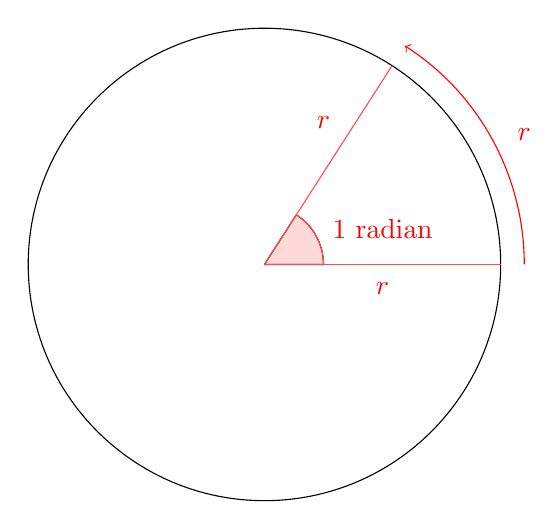
\begin{tikzpicture}[yscale=1,xscale=1,scale=1.5,inner sep=0.1mm, label distance=1.5mm]

%\draw[black!30!white, ->] (-3,0) -- (3,0);
%\draw[black!30!white, ->] (0,-3) -- (0,3);
%\node(t) at (3.15,0) [color=black!50!white] {$x$};
%\node(t) at (0,3.15) [color=black!50!white] {$y$};
\draw (0,0) circle (2);
\draw[fill=red!15!white] (0,0) -- (0.5,0) arc (0:57.2958:0.5cm)  -- (0,0);
\draw[color=red!70!white] (0.5,0) arc (0:57.2958:0.5cm);
\draw[red!70!white] (0,0) -- (2,0);
\draw[red!70!white] (0,0) -- (1.08060461174,1.68294196962);
\draw[red, ->] (2.2,0) arc (0:57.2958:2.2cm);
\node(l) at (2.2,1.1) [color=red] {$r$};
\node(r) at (1,-0.2) [color=red] {$r$};
\node(j) at (0.5,1.2) [color=red] {$r$};
\node(j) at (1,0.3) [color=red] {$1$ radian};

\end{tikzpicture}

\end{document}